\documentclass{article}

\usepackage[final]{style}
\usepackage[utf8]{inputenc} % allow utf-8 input
\usepackage[T1]{fontenc}    % use 8-bit T1 fonts
\usepackage{hyperref}       % hyperlinks
\usepackage{url}            % simple URL typesetting
\usepackage{booktabs}       % professional-quality tables
\usepackage{amsfonts}       % blackboard math symbols
\usepackage{nicefrac}       % compact symbols for 1/2, etc.
\usepackage{microtype}      % microtypography
\usepackage{verbatim}
\usepackage{graphicx}       % for figures
\usepackage{amsmath}

\title{Lecture \#6-7: Features and Fitting/Feature Descriptors}

\author{
  Trevor Danielson, Wesley Olmsted, Kelsey Wang, Ben Barnett \\
  Department of Computer Science\\
  Stanford University\\
  Stanford, CA 94305 \\
  \texttt{\{trevord, wolmsted, kyw, ben.barnett\}@cs.stanford.edu} \\
}

\begin{document}

\maketitle


% RANSAC - Ben Barnett (barnett3)
\section{RANSAC}
\subsection{Goal}
RANdom SAmple Consensus (RANSAC) is used for model fitting in images (e.g., line detection); it can be extremely useful for object identification, among other applications. It is often more effective than pure edge detection which is prone to several limitations: edges containing extra points due to the noise/clutter, certain parts of the edges being left out, and the existence of noise in measured edges' orientation.
\subsection{Motivation}
One of the primary advantages of RANSAC is that it is relatively efficient and accurate even when the number of parameters is high. However, it should be noted that RANSAC is likely to fail or produce inaccurate results in images with a relatively large amount of noise.
\subsection{General Approach}
The intuition for RANSAC is that by randomly sampling a group of points in an edge and applying a line of best fit to those points \textit{many times}, we have a high probability of finding a line that fits the points very well. Below is the general process "RANSAC loop":
\begin{enumerate}
\item Randomly select a seed group of points from the overall group of points you are trying to fit with a line.
\item Compute a line of best fit among the seed group. For example, if the seed group is only 2 distinct points, then it is clear to see that there is only one line that passes through both points, which can be determined with relative ease from the points' coordinates.
\item Find the number of \textbf{inliers} to this line by iterating over each point in the data set and calculating its distance from the line; if is less than a (predetermined) threshold value, it counts as an inlier. Otherwise, it is counted as an outlier.
\item If the number of inliers is sufficiently large, conclude that this line is "good", and that at least one line exists that includes the inliers tallied in the previous step. To further improve the line, re-compute the line using a least-squares estimate using all of the inliers that were within the threshold distance. Keep this transformation as the line that best approximates the data.
\end{enumerate}
\subsection{Drawbacks}
The biggest drawback to RANSAC is its inefficient handling of highly noisy data; an increase in the fraction of outliers in a given data set results in an increase in the number of samples required for model fitting (e.g., line of best fit). More importantly, the noisier an image is, the less likely it is for a line to \textit{ever} be considered sufficiently good at fitting the data. This is a significant problem because most real world problems have a relatively large proportion of noise/outliers.


% LOCAL INVARIANT FEATURES - Trevor Danielson
\section{Local Invariant Features}
\subsection{Motivation}
\paragraph{} The local invariant image features and their descriptors are used in a wide range of computer vision applications; they include, but are not limited to, object detection, classification, tracking, motion estimation, panorama stitching, and image registration. The previously discussed methods, such as cross-correlation, are not effective and robust in many of such appl. This method works by finding local, distinctive structures within an image (i.e., features), and it describes each feature using the surrounding region (e.g., a small patch centered on the detected feature). This "local" representation of image features (as opposed to a "global" one, such as cross-correlation) provides a more robust means of addressing the above-mentioned computer vision problems; such strategy is invariant to object rotations, point of view translations, and scale changes.

\subsection{General Approach}
The general approach for employing local invariant features is detailed below:
\begin{enumerate}
\item Find and define a set of distinctive keypoints.
\item Define a local region around the keypoint.
\item Extract and normalize the regional content from the area.
\item Compute a local descriptor from the normalized region (i.e., a function of pixel intensity).
\item Match local descriptors.
\end{enumerate}
\begin{center}
	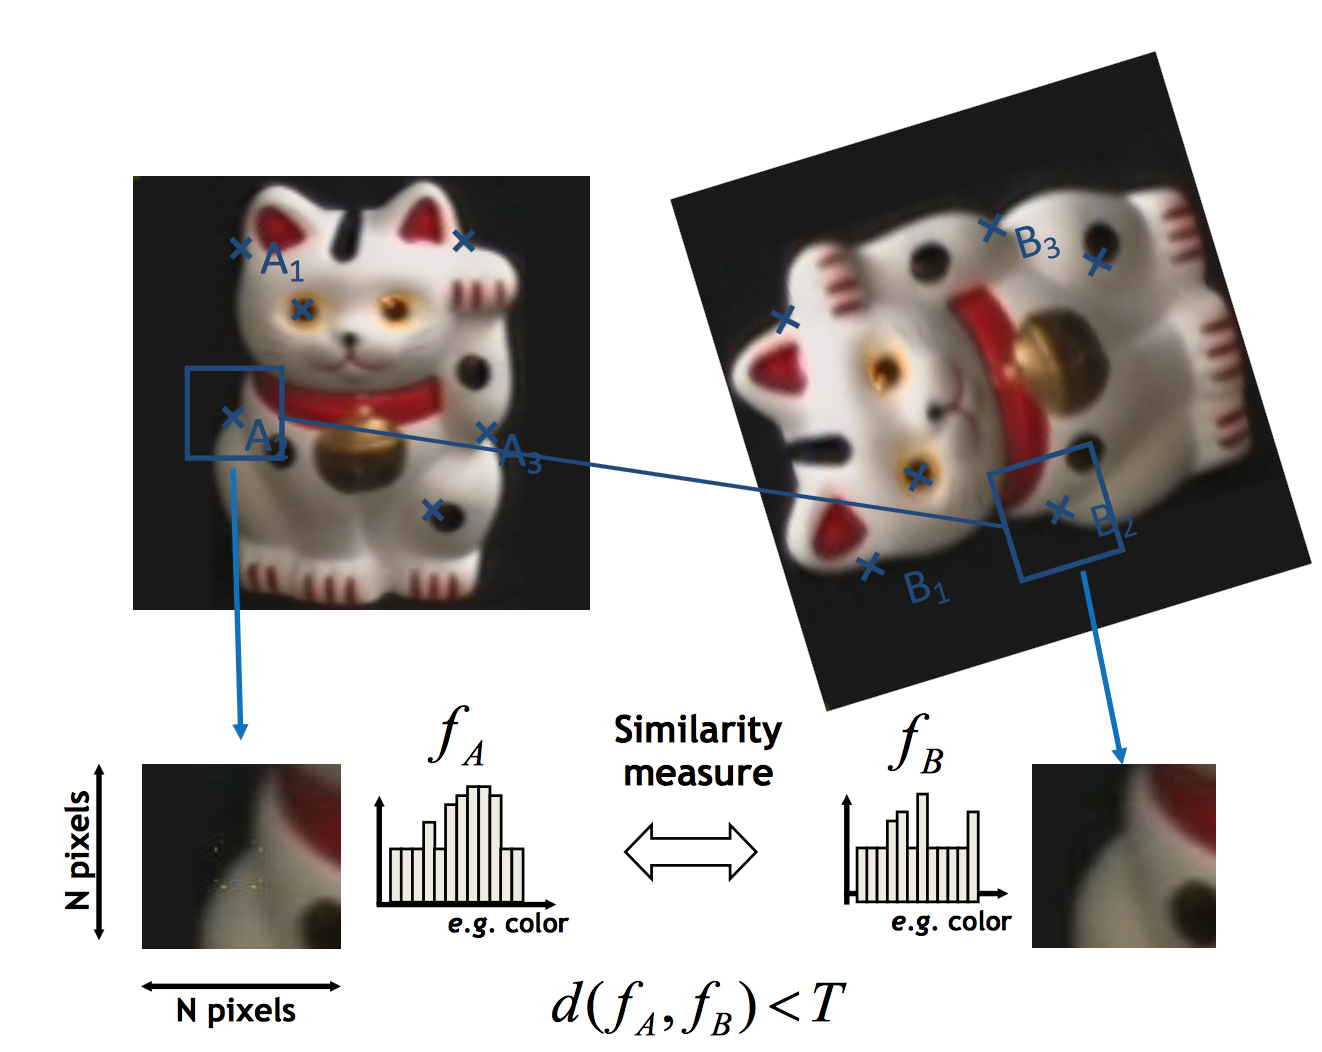
\includegraphics[scale=0.5]{local_feature_ex.png}\\
  	\textbf{Figure 1:} The local features are identified within similar pictures; descriptors are calculated for normalized patches and compared to each other for quantifying the similarity. Source: Lecture 6 slides. \\
\end{center}
\subsection{Requirements}
Good local features should have the following properties:
\begin{enumerate}
\item \textit{Repeatability}: given the same object or scene under different image conditions such as lighting or change in viewpoint, a high amount of features should be detectable in both images being compared. In other words, the feature detection should be invariant to rotations and viewpoint changes and robustly handle lighting changes, noise, and blur.
\item \textit{Locality}: features should be local to avoid issues caused by occlusion and clutter.
\item \textit{Quantity}: enough features should be chosen to ensure the accuracy of techniques relying on descriptors such as object detection.
\item \textit{Distinctiveness}: results need to contain "salient" image features that show a large amount of variation; this ensures that the detected features can be distinguished from each other and properly matched between different images.
\item \textit{Efficiency}: feature matching in new images should be conducive to real-time applications.
\end{enumerate}

%Keypoint Localization - Kelsey Wang
\section{Keypoint Localization}
\subsection{Motivation}
\paragraph{} The goal of keypoint localization is to detect features consistently and repeatedly, to allow for more precise localization, and to find interesting content within the image.

\subsection{General Approach}
We will look for corners since they are repeatable and distinctive in the majority of images. To find corners, we look for large changes in intensity in all directions. To provide context, a "flat" region would not have change in any direction, and an edge would have no change along the direction of the edge. We will find these corners using the Harris technique.

\subsection{Harris Detector}
The intuition behind Harris detector is that if a window ($w$) slides over an image, the change in the intensity of pixel values caused by the shift is highest at corners. This is because change in pixel intensity is observed in both directions ($x$ and $y$) at corners, while it is limited to only one direction at the edges, and it is negligible at flat image regions.  To calculate the change of intensity due to the shift $[u,v]$:
$$E(u,v) = \sum_{x,y}^{} w(x,y)[I(x+u,y+v)-I(x,y)]^2$$
To find corners, we must maximize this function. Taylor Expansion is then used in the process to get the following equation:
\[
E(u,v)=
  \begin{bmatrix}
    u & v\\
  \end{bmatrix}
  M
  \begin{bmatrix}
      u \\
      v
    \end{bmatrix}
\]
where we have M defined as:
\[M =
\sum_{x,y}^{} w(x,y)
  \begin{bmatrix}
      I_x I_x & I_x I_y\\
      I_x I_y & I_y I_y
    \end{bmatrix}
\]
This matrix reveals:
\[M =
  \begin{bmatrix}
      \sum I_x I_x & \sum I_x I_y\\
      \sum I_x I_y & \sum I_y I_y
    \end{bmatrix}
    =
    \begin{bmatrix}
      \lambda_1 & 0\\
      0 & \lambda_2
    \end{bmatrix}
\]
Corners have both large and similar eigenvalues, whereas edges have one significantly greater eigenvalue, and flat regions have two small eigenvalues. Because the calculation of eigenvalues is computationally intensive, an alternative approach is employed where the Corner Response Function ($\theta$) is used to compute a score for each window:
$$\theta = det(M) - \alpha \textnormal{trace} (M)^2 $$
where $\alpha$ is a constant around $.04-.06$.
\begin{center}
	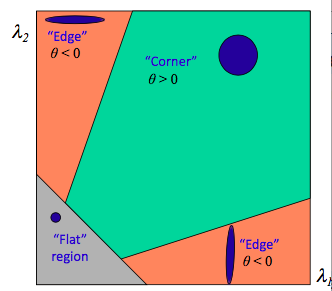
\includegraphics[scale=0.5]{eigenvalues_harris.png}\\
    \textbf{Figure 2:} The visualization of theta thresholds from Corner Response Function ($\theta$) indicating corner, edge, or flat regions. Source: Lecture 6 slides\\
\end{center}

This is not rotation invariant. To allow for rotation invariance, we will smooth with Gaussian, where the Gaussian already performs the weighted sum:

\[M =
g( \sigma )
  \begin{bmatrix}
      I_x I_x & I_x I_y\\
      I_x I_y & I_y I_y
    \end{bmatrix}
\]

Illustrated below is an of keypoints identified by Harris detector.
\begin{center}
	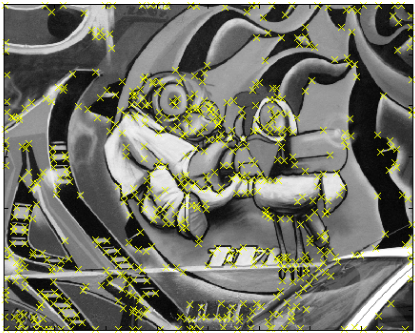
\includegraphics[scale=0.5]{harris_response.png}\\
    \textbf{Figure 3:} An example of Harris keypoint detection on an image. Source: Lecture 6 slides \\
\end{center}

%Scale invariant keypoint detection - Wesley Olmsted
\section{Scale Invariant Keypoint Detection}
\subsection{Motivation}
Earlier we used the Harris detector to find keypoints or corners. This detector used small windows in order to maintain good locality. Since the Harris detector uses this small window, if an image is scaled up, the window now no longer sees the same gradients it had with a smaller image.\\
\begin{center}
	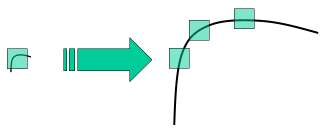
\includegraphics{sift_scale_invariant.jpg} \\
    \textbf{Figure 4:} Harris detector windows on an increased scale. Source: \cite{opencv}
\end{center}
Figure 4:
Looking at the above image, we can see how the three windows on the right no longer see the sharp gradient in the x and y directions. All three windows are, therefore, classified edges. In order to address this problem, we need to normalize the scale of the detector.
\subsection{Solution}
We design a function to be scale-invariant, meaning that the function values for the corresponding regions are the same regardless of the scale. We can use a circle to represent this scalable function. A point on the circle is a function of the region size of the circle's radius.
\subsection{General Approach}
We can find the local maximum of a function. Relative to the local maximum, the region size should be the same regardless of the scale. This also means that the region size is co-variant with the image scale. A "good" function results in a single and distinct local maximum. In general, we should use a function that responds well to stark contrasts in intensity. \\
\begin{center}
	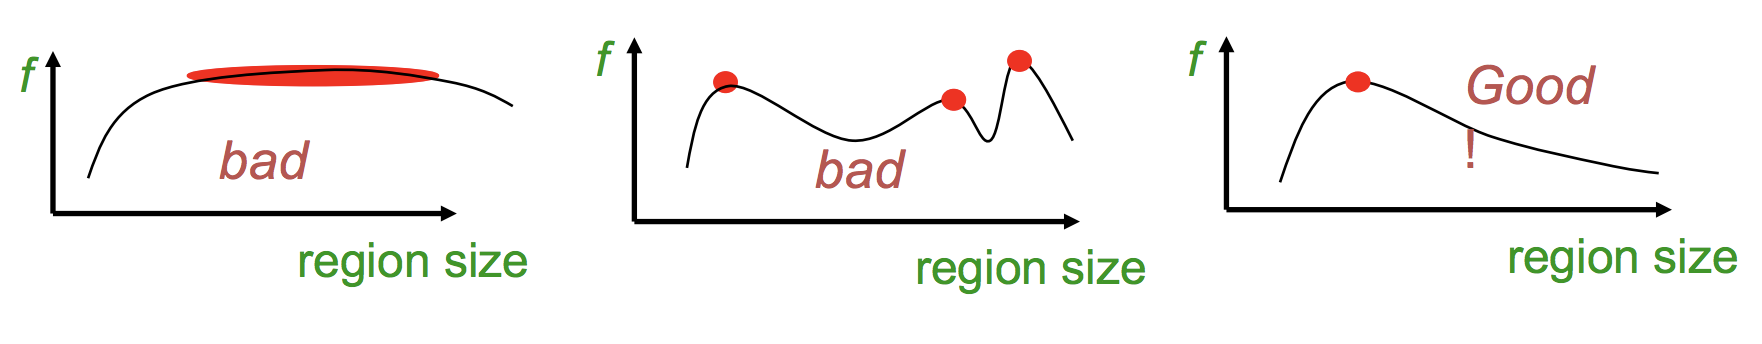
\includegraphics[scale=0.5]{scaleinvariant.png}\\
    \textbf{Figure 5:} The examples of different functions for finding local maximums. Source: Lecture 7 slides.
\end{center}
The function is defined as: $f = kernel*image$. Two such kernels include the Laplacian and the Difference of Gaussians (DoG). $$L = \sigma^2(G_{xx}(x,y,\sigma)+G_{yy}(x,y,\sigma))$$ $$DoG = G(x,y,k\sigma) - G(x,y,\sigma)$$ $$G(x,y,\sigma) = \frac{1}{\sqrt{2\pi}\sigma}e^{-\frac{x^2+y^2}{2\sigma^2}}$$
Both these kernels are scale and rotation invariant.




% References
\small
\bibliographystyle{plain}
\bibliography{bibliography}
\end{document}
